%%%% University of Cambridge tech-report formatting; enable when producing
%%%% tech-report versions of these documents; otherwise, disable.
\documentclass[12pt,twoside,openright,a4paper]{article}
\setlength{\oddsidemargin}{-0.4mm} % 25 mm left margin
\setlength{\evensidemargin}{\oddsidemargin}
\setlength{\textwidth}{160mm}      % 25 mm right margin
\setlength{\topmargin}{-5.4mm}     % 20 mm top margin
\setlength{\headheight}{5mm}
\setlength{\headsep}{5mm}
\setlength{\footskip}{10mm}
\setlength{\textheight}{237mm}     % 20 mm bottom margin
%%%% .. or regular document
%\documentclass[12pt,letterpaper,twoside,openright,fleqn]{report}
%%%% End of tech-report vs. regular
%%%%

\usepackage{graphicx}

\begin{document}

\title{PVMv2 Specification}
\author{Thomas Bytheway & Lucian Carata}

%% CL tech-report format provides its own cover page
\begin{minipage}[h]{\textwidth}
    \maketitle
    \vspace{2in}
    {\small}
\end{minipage}
%%

\normalsize

%% CL tech-report format requires page numbering to start at 3
%\setcounter{page}{3}
%%

%% For revisions sent for editing, prefer double spacing.
%\doublespacing
%%

\clearpage

\section{Introduction}

\section{Types}

\subsection{Entities}
\begin{figure}[h]
\centering
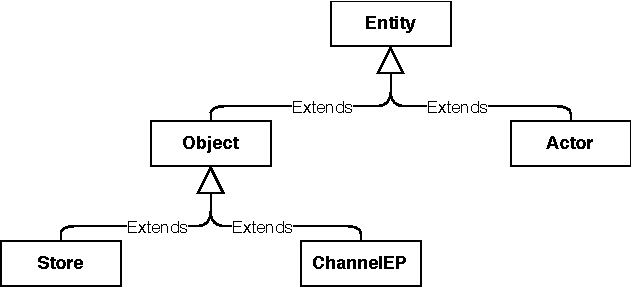
\includegraphics{pvm_types.pdf}
\caption{A diagram of the basic abstract types in PVMv2}
\end{figure}

\paragraph{Entity}

\paragraph{Actor}
Active entities that perform actions. They act upon objects, or other actors. Generally processing elements like unix processes.

\paragraph{Object}
Passive entities that are acted upon by actors. Generally data carrying entities.

\paragraph{Store}
Object type that stores data internally. Versions from first write to last write, using EditSessions.

\paragraph{ChannelEP}
Object type that data flows through without internal storage. Does not version. May participate in connections.

\subsection{Non-canonical Names}

\section{Relations}

\paragraph{INF}
Indicates that the source has potentially imparted data or control to the destination.

\paragraph{NAMED}
Indicates that the source has been mentioned by the destination non-canonical name.

\section{Mappings}

\subsection{Concrete Type Declaration}

\subsection{Verbs}

\paragraph{Declare}
Forces the creation of entity if it does not already exist.

\paragraph{Sink}
Called when as part of a mapped function, an actor sinks data to an entity as an ‘atomic’ operation.
Causes Files to version, creating a new File entity connected to the previous one by an INF relation.
Creates an INF relation from actor to entity, attaching tag as the ‘type’ property. 

\paragraph{Source}
Called when as part of a mapped function, an actor sources data from an entity.
Creates an INF relation from entity to actor, attaching tag as the ‘type’ property.

\paragraph{Connect}
Called as part of a mapped function to declare that two conduit nodes are connected to each other and that data can flow between them. The dir argument indicates the direction of flow, either mono or bi. Mono indicates that data may only flow from the first conduit to the second, bi indicates that data may flow in both directions. 

\paragraph{Mention}

\paragraph{Unlink}

\paragraph{Property}

\end{document}
